%Do not change 
\documentclass[12pt, oneside]{article}
\usepackage{amssymb,amsmath}
\usepackage[margin=1in]{geometry}
\usepackage{textpos}
\usepackage{float}
%\usepackage{color}
\usepackage{graphicx}
\usepackage{tikz}
\usetikzlibrary{positioning}
\usepackage{tikz-3dplot}
\usepackage{pgfopts}
\usepackage{wasysym}
\usepackage{structuralanalysis}
\usepackage{fancyhdr}
\usepackage[en-US]{datetime2}

\fancyhead[R]{\small Last Updated: \today\ at \DTMcurrenttime}
\pagestyle{fancy}

% You may add the packages you need here



\begin{document}
% Do not modify 


%Do not modify
\begin{textblock*}{4cm}(-1.7cm,-2.3cm)
\noindent {\scriptsize AE737 Spring 2016} 
\end{textblock*}

%Do not modify other than putting your name where stated
\begin{textblock*}{8cm}(12.5cm,-1cm)
\noindent {Name: } 
\end{textblock*}
%Do not modify other than typing your acknowledgement where stated
\begin{textblock*}{13.5cm}(-1.7cm,-1.8cm)
%\noindent \textit{\footnotesize Acknowledgement: Your acknowledgement for collaboration and other sources goes here. } 
\end{textblock*}

\vspace{1cm}

%Do not modify other than typing the homework number after #
\begin{center}
\textbf{\Large Homework 2}

\textbf{Due 9 Feb 2016}
\end{center}


%Rest should contain your solution for the homework. Feel free to improvise in ways that you believe make grading easier.
\begin{enumerate}

\begin{figure}[H]
	\item Determine the stress intensity for the edge cracked panel ($\sigma_{YS} = 75 \text{ ksi}$)
	\begin{enumerate}
		\item Without any plastic zone adjustment
		\item With a plane stress plastic zone adjustment
		\item With a plane strain plastic zone adjustment
		\item For $t = 0.125"$
	\end{enumerate}
		\centering
		\begin{tikzpicture}
		\begin{scope}[scale=.5]
		\draw (0,-3) -- (0,3) -- (8,3) -- (8,-3) -- (0,-3);
		\draw[->] (4,3) -- (4,4) node[above] {12 ksi};
		\draw[->] (4,-3) -- (4,-4) node[below] {12 ksi};
		\draw (0,0) -- (2,0);
		\draw node at (1.2,0.5) {2"};
		\draw[->] (3.5,-2.5) -- (0,-2.5);
		\draw[->] (4.5,-2.5) -- (8,-2.5);
		\draw node at (4,-2.5) {8"};
		\end{scope}
		\end{tikzpicture}
\end{figure}

\begin{figure}[H]
	\item Plot effective (plastic) stress intensity over elastic stress intensity vs. applied stress over yield stress ($K_e/K \text{ vs. } \sigma/\sigma_{YS}$) for an infinitely wide center-cracked panel in plane strain.
\end{figure}

\begin{figure}[H]
	\item Determine $K_e/K$ for a finite width center cracked panel in the following cases ($\sigma = 30 \text{ ksi}$, $\sigma_{YS} = 65 \text{ ksi}$, )
	\begin{enumerate}
		\item $2a = 2\text{"}$, $W = 8 \text{"}$, plane strain
		\item $2a = 2\text{"}$, $W = 5 \text{"}$, plane stress
		\item $2a = 2\text{"}$, $W = 5 \text{"}$, plot for varying thickness, 1/16" to 5/8"
	\end{enumerate}
\end{figure}

\begin{figure}[H]
	\item Plot the plastic zone shape according the structure shown ($\sigma_{YS} = 50 \text{ ksi}$, $\nu = 0.33$).
	\begin{enumerate}
		\item Plane stress, Von Mises Yield Theory
		\item Plane strain, Von Mises Yield Theory
		\item Plane stress, Tresca Yield Criteria
		\item Plane strain, Tresca Yield Criteria
	\end{enumerate}
	\centering
	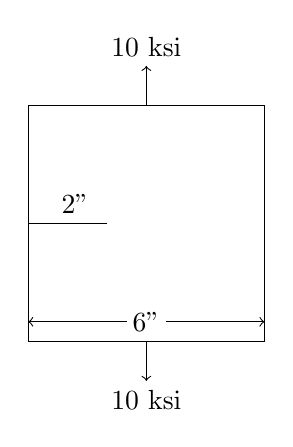
\begin{tikzpicture}
	\begin{scope}[scale=.5]
	\draw (0,-3) -- (0,3) -- (6,3) -- (6,-3) -- (0,-3);
	\draw[->] (3,3) -- (3,4) node[above] {10 ksi};
	\draw[->] (3,-3) -- (3,-4) node[below] {10 ksi};
	\draw (0,0) -- (2,0);
	\draw node at (1.2,0.5) {2"};
	\draw[->] (2.5,-2.5) -- (0,-2.5);
	\draw[->] (3.5,-2.5) -- (6,-2.5);
	\draw node at (3,-2.5) {6"};
	\end{scope}
	\end{tikzpicture}
\end{figure}

\end{enumerate}
\end{document}
